% Created by tikzDevice version 0.12.3.1 on 2022-05-05 15:47:27
% !TEX encoding = UTF-8 Unicode
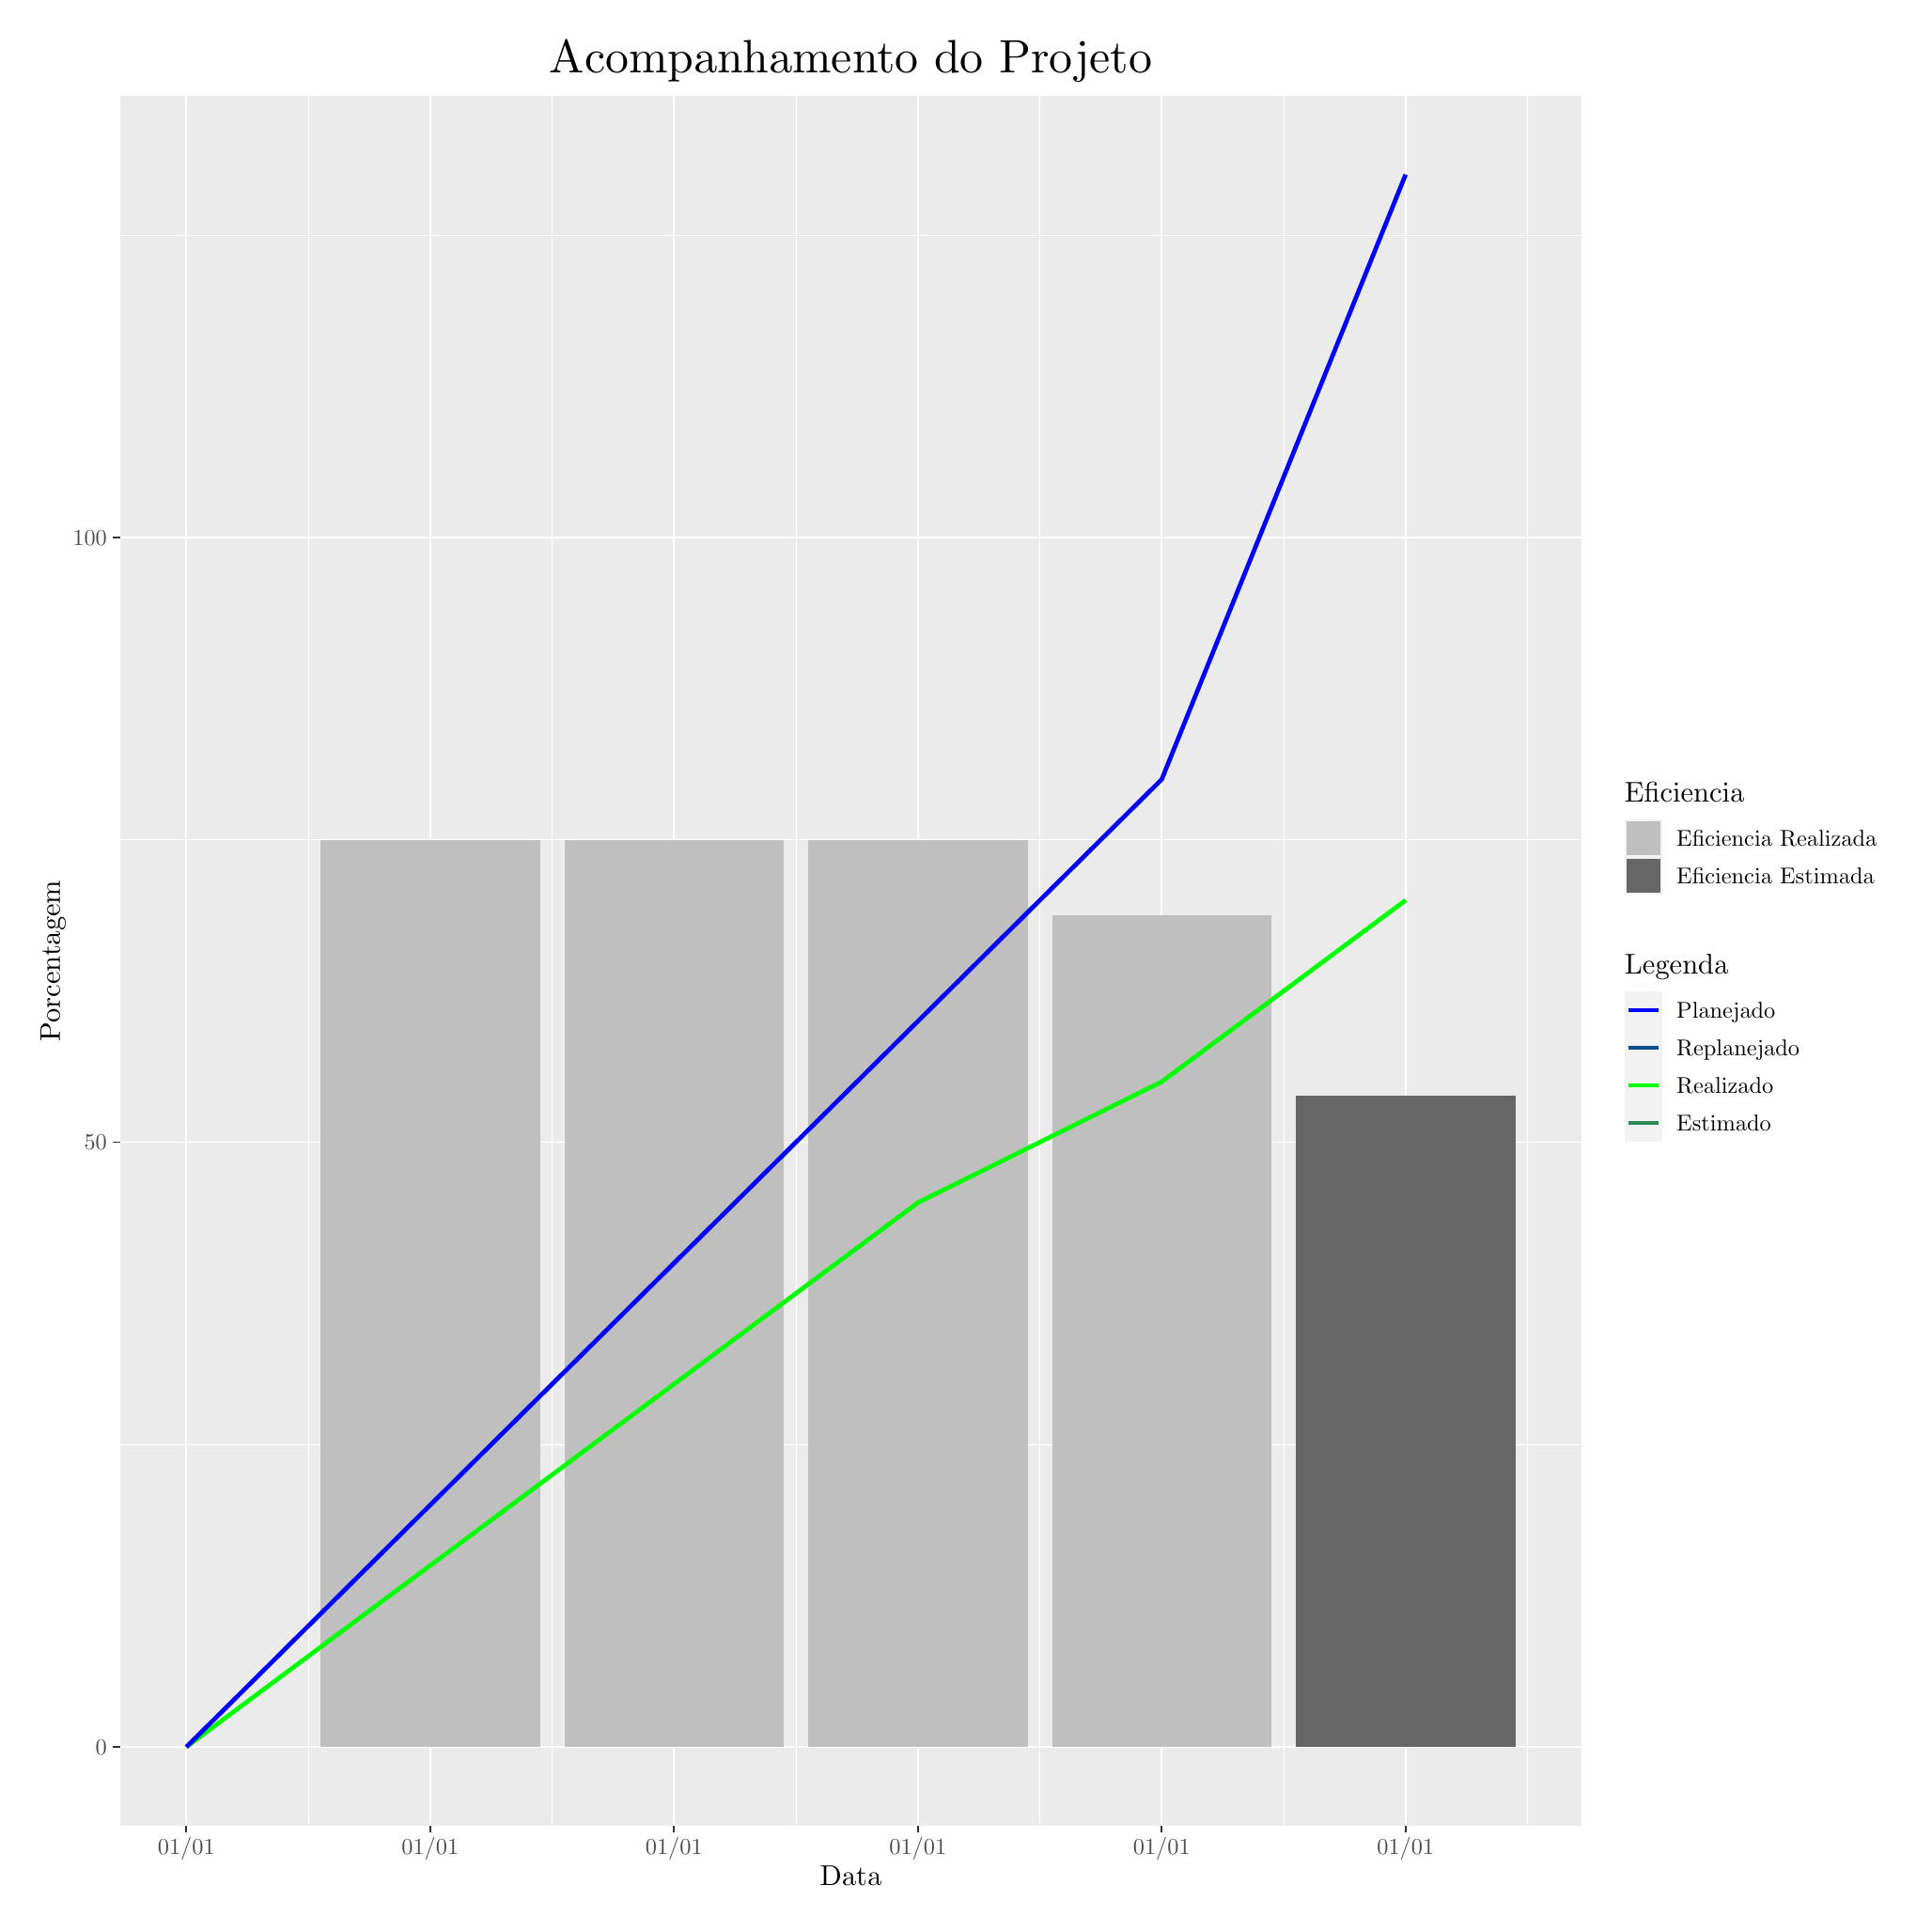
\begin{tikzpicture}[x=1pt,y=1pt]
\definecolor{fillColor}{RGB}{255,255,255}
\path[use as bounding box,fill=fillColor,fill opacity=0.00] (0,0) rectangle (722.70,722.70);
\begin{scope}
\path[clip] (  0.00,  0.00) rectangle (722.70,722.70);
\definecolor{drawColor}{RGB}{255,255,255}
\definecolor{fillColor}{RGB}{255,255,255}

\path[draw=drawColor,line width= 0.6pt,line join=round,line cap=round,fill=fillColor] (  0.00,  0.00) rectangle (722.70,722.70);
\end{scope}
\begin{scope}
\path[clip] ( 36.11, 30.69) rectangle (598.26,695.80);
\definecolor{fillColor}{gray}{0.92}

\path[fill=fillColor] ( 36.11, 30.69) rectangle (598.26,695.80);
\definecolor{drawColor}{RGB}{255,255,255}

\path[draw=drawColor,line width= 0.3pt,line join=round] ( 36.11,177.20) --
	(598.26,177.20);

\path[draw=drawColor,line width= 0.3pt,line join=round] ( 36.11,409.76) --
	(598.26,409.76);

\path[draw=drawColor,line width= 0.3pt,line join=round] ( 36.11,642.32) --
	(598.26,642.32);

\path[draw=drawColor,line width= 0.3pt,line join=round] (108.55, 30.69) --
	(108.55,695.80);

\path[draw=drawColor,line width= 0.3pt,line join=round] (202.32, 30.69) --
	(202.32,695.80);

\path[draw=drawColor,line width= 0.3pt,line join=round] (296.09, 30.69) --
	(296.09,695.80);

\path[draw=drawColor,line width= 0.3pt,line join=round] (389.86, 30.69) --
	(389.86,695.80);

\path[draw=drawColor,line width= 0.3pt,line join=round] (483.63, 30.69) --
	(483.63,695.80);

\path[draw=drawColor,line width= 0.3pt,line join=round] (577.40, 30.69) --
	(577.40,695.80);

\path[draw=drawColor,line width= 0.6pt,line join=round] ( 36.11, 60.92) --
	(598.26, 60.92);

\path[draw=drawColor,line width= 0.6pt,line join=round] ( 36.11,293.48) --
	(598.26,293.48);

\path[draw=drawColor,line width= 0.6pt,line join=round] ( 36.11,526.04) --
	(598.26,526.04);

\path[draw=drawColor,line width= 0.6pt,line join=round] ( 61.66, 30.69) --
	( 61.66,695.80);

\path[draw=drawColor,line width= 0.6pt,line join=round] (155.43, 30.69) --
	(155.43,695.80);

\path[draw=drawColor,line width= 0.6pt,line join=round] (249.20, 30.69) --
	(249.20,695.80);

\path[draw=drawColor,line width= 0.6pt,line join=round] (342.97, 30.69) --
	(342.97,695.80);

\path[draw=drawColor,line width= 0.6pt,line join=round] (436.74, 30.69) --
	(436.74,695.80);

\path[draw=drawColor,line width= 0.6pt,line join=round] (530.52, 30.69) --
	(530.52,695.80);
\definecolor{fillColor}{gray}{0.75}

\path[fill=fillColor] (113.24, 60.92) rectangle (197.63,409.76);

\path[fill=fillColor] (207.01, 60.92) rectangle (291.40,409.76);

\path[fill=fillColor] (300.78, 60.92) rectangle (385.17,409.76);

\path[fill=fillColor] (394.55, 60.92) rectangle (478.94,380.69);

\path[fill=fillColor] (488.32, 60.92) rectangle (572.71,311.37);
\definecolor{fillColor}{gray}{0.40}

\path[fill=fillColor] (488.32, 60.92) rectangle (572.71,311.37);
\definecolor{drawColor}{RGB}{0,255,0}

\path[draw=drawColor,line width= 1.7pt,line join=round] ( 61.66, 60.92) --
	(155.43,130.69) --
	(249.20,200.45) --
	(342.97,270.22) --
	(436.74,316.73) --
	(530.52,386.50);
\definecolor{drawColor}{RGB}{0,0,255}

\path[draw=drawColor,line width= 1.7pt,line join=round] ( 61.66, 60.92) --
	(155.43,153.94) --
	(249.20,246.97) --
	(342.97,339.99) --
	(436.74,433.01) --
	(530.52,665.57);
\end{scope}
\begin{scope}
\path[clip] (  0.00,  0.00) rectangle (722.70,722.70);
\definecolor{drawColor}{gray}{0.30}

\node[text=drawColor,anchor=base east,inner sep=0pt, outer sep=0pt, scale=  0.88] at ( 31.16, 57.89) {0};

\node[text=drawColor,anchor=base east,inner sep=0pt, outer sep=0pt, scale=  0.88] at ( 31.16,290.45) {50};

\node[text=drawColor,anchor=base east,inner sep=0pt, outer sep=0pt, scale=  0.88] at ( 31.16,523.01) {100};
\end{scope}
\begin{scope}
\path[clip] (  0.00,  0.00) rectangle (722.70,722.70);
\definecolor{drawColor}{gray}{0.20}

\path[draw=drawColor,line width= 0.6pt,line join=round] ( 33.36, 60.92) --
	( 36.11, 60.92);

\path[draw=drawColor,line width= 0.6pt,line join=round] ( 33.36,293.48) --
	( 36.11,293.48);

\path[draw=drawColor,line width= 0.6pt,line join=round] ( 33.36,526.04) --
	( 36.11,526.04);
\end{scope}
\begin{scope}
\path[clip] (  0.00,  0.00) rectangle (722.70,722.70);
\definecolor{drawColor}{gray}{0.20}

\path[draw=drawColor,line width= 0.6pt,line join=round] ( 61.66, 27.94) --
	( 61.66, 30.69);

\path[draw=drawColor,line width= 0.6pt,line join=round] (155.43, 27.94) --
	(155.43, 30.69);

\path[draw=drawColor,line width= 0.6pt,line join=round] (249.20, 27.94) --
	(249.20, 30.69);

\path[draw=drawColor,line width= 0.6pt,line join=round] (342.97, 27.94) --
	(342.97, 30.69);

\path[draw=drawColor,line width= 0.6pt,line join=round] (436.74, 27.94) --
	(436.74, 30.69);

\path[draw=drawColor,line width= 0.6pt,line join=round] (530.52, 27.94) --
	(530.52, 30.69);
\end{scope}
\begin{scope}
\path[clip] (  0.00,  0.00) rectangle (722.70,722.70);
\definecolor{drawColor}{gray}{0.30}

\node[text=drawColor,anchor=base,inner sep=0pt, outer sep=0pt, scale=  0.88] at ( 61.66, 19.68) {01/01};

\node[text=drawColor,anchor=base,inner sep=0pt, outer sep=0pt, scale=  0.88] at (155.43, 19.68) {01/01};

\node[text=drawColor,anchor=base,inner sep=0pt, outer sep=0pt, scale=  0.88] at (249.20, 19.68) {01/01};

\node[text=drawColor,anchor=base,inner sep=0pt, outer sep=0pt, scale=  0.88] at (342.97, 19.68) {01/01};

\node[text=drawColor,anchor=base,inner sep=0pt, outer sep=0pt, scale=  0.88] at (436.74, 19.68) {01/01};

\node[text=drawColor,anchor=base,inner sep=0pt, outer sep=0pt, scale=  0.88] at (530.52, 19.68) {01/01};
\end{scope}
\begin{scope}
\path[clip] (  0.00,  0.00) rectangle (722.70,722.70);
\definecolor{drawColor}{RGB}{0,0,0}

\node[text=drawColor,anchor=base,inner sep=0pt, outer sep=0pt, scale=  1.10] at (317.19,  7.64) {Data};
\end{scope}
\begin{scope}
\path[clip] (  0.00,  0.00) rectangle (722.70,722.70);
\definecolor{drawColor}{RGB}{0,0,0}

\node[text=drawColor,rotate= 90.00,anchor=base,inner sep=0pt, outer sep=0pt, scale=  1.10] at ( 13.08,363.24) {Porcentagem};
\end{scope}
\begin{scope}
\path[clip] (  0.00,  0.00) rectangle (722.70,722.70);
\definecolor{fillColor}{RGB}{255,255,255}

\path[fill=fillColor] (609.26,383.20) rectangle (717.20,438.32);
\end{scope}
\begin{scope}
\path[clip] (  0.00,  0.00) rectangle (722.70,722.70);
\definecolor{drawColor}{RGB}{0,0,0}

\node[text=drawColor,anchor=base west,inner sep=0pt, outer sep=0pt, scale=  1.10] at (614.76,424.18) {Eficiencia};
\end{scope}
\begin{scope}
\path[clip] (  0.00,  0.00) rectangle (722.70,722.70);
\definecolor{fillColor}{gray}{0.95}

\path[fill=fillColor] (614.76,403.15) rectangle (629.22,417.61);
\end{scope}
\begin{scope}
\path[clip] (  0.00,  0.00) rectangle (722.70,722.70);
\definecolor{fillColor}{gray}{0.75}

\path[fill=fillColor] (615.48,403.86) rectangle (628.51,416.90);
\end{scope}
\begin{scope}
\path[clip] (  0.00,  0.00) rectangle (722.70,722.70);
\definecolor{fillColor}{gray}{0.75}

\path[fill=fillColor] (615.48,403.86) rectangle (628.51,416.90);
\end{scope}
\begin{scope}
\path[clip] (  0.00,  0.00) rectangle (722.70,722.70);
\definecolor{fillColor}{gray}{0.95}

\path[fill=fillColor] (614.76,388.70) rectangle (629.22,403.15);
\end{scope}
\begin{scope}
\path[clip] (  0.00,  0.00) rectangle (722.70,722.70);
\definecolor{fillColor}{gray}{0.40}

\path[fill=fillColor] (615.48,389.41) rectangle (628.51,402.44);
\end{scope}
\begin{scope}
\path[clip] (  0.00,  0.00) rectangle (722.70,722.70);
\definecolor{fillColor}{gray}{0.40}

\path[fill=fillColor] (615.48,389.41) rectangle (628.51,402.44);
\end{scope}
\begin{scope}
\path[clip] (  0.00,  0.00) rectangle (722.70,722.70);
\definecolor{drawColor}{RGB}{0,0,0}

\node[text=drawColor,anchor=base west,inner sep=0pt, outer sep=0pt, scale=  0.88] at (634.72,407.35) {Eficiencia Realizada};
\end{scope}
\begin{scope}
\path[clip] (  0.00,  0.00) rectangle (722.70,722.70);
\definecolor{drawColor}{RGB}{0,0,0}

\node[text=drawColor,anchor=base west,inner sep=0pt, outer sep=0pt, scale=  0.88] at (634.72,392.90) {Eficiencia Estimada};
\end{scope}
\begin{scope}
\path[clip] (  0.00,  0.00) rectangle (722.70,722.70);
\definecolor{fillColor}{RGB}{255,255,255}

\path[fill=fillColor] (609.26,288.17) rectangle (687.51,372.20);
\end{scope}
\begin{scope}
\path[clip] (  0.00,  0.00) rectangle (722.70,722.70);
\definecolor{drawColor}{RGB}{0,0,0}

\node[text=drawColor,anchor=base west,inner sep=0pt, outer sep=0pt, scale=  1.10] at (614.76,358.05) {Legenda};
\end{scope}
\begin{scope}
\path[clip] (  0.00,  0.00) rectangle (722.70,722.70);
\definecolor{fillColor}{gray}{0.95}

\path[fill=fillColor] (614.76,337.03) rectangle (629.22,351.48);
\end{scope}
\begin{scope}
\path[clip] (  0.00,  0.00) rectangle (722.70,722.70);
\definecolor{drawColor}{RGB}{0,0,255}

\path[draw=drawColor,line width= 1.7pt,line join=round] (616.21,344.26) -- (627.77,344.26);
\end{scope}
\begin{scope}
\path[clip] (  0.00,  0.00) rectangle (722.70,722.70);
\definecolor{drawColor}{RGB}{0,0,255}

\path[draw=drawColor,line width= 1.7pt,line join=round] (616.21,344.26) -- (627.77,344.26);
\end{scope}
\begin{scope}
\path[clip] (  0.00,  0.00) rectangle (722.70,722.70);
\definecolor{drawColor}{RGB}{0,0,255}

\path[draw=drawColor,line width= 1.7pt,line join=round] (616.21,344.26) -- (627.77,344.26);
\end{scope}
\begin{scope}
\path[clip] (  0.00,  0.00) rectangle (722.70,722.70);
\definecolor{drawColor}{RGB}{0,0,255}

\path[draw=drawColor,line width= 1.7pt,line join=round] (616.21,344.26) -- (627.77,344.26);
\end{scope}
\begin{scope}
\path[clip] (  0.00,  0.00) rectangle (722.70,722.70);
\definecolor{fillColor}{gray}{0.95}

\path[fill=fillColor] (614.76,322.58) rectangle (629.22,337.03);
\end{scope}
\begin{scope}
\path[clip] (  0.00,  0.00) rectangle (722.70,722.70);
\definecolor{drawColor}{RGB}{16,78,139}

\path[draw=drawColor,line width= 1.7pt,line join=round] (616.21,329.80) -- (627.77,329.80);
\end{scope}
\begin{scope}
\path[clip] (  0.00,  0.00) rectangle (722.70,722.70);
\definecolor{drawColor}{RGB}{16,78,139}

\path[draw=drawColor,line width= 1.7pt,line join=round] (616.21,329.80) -- (627.77,329.80);
\end{scope}
\begin{scope}
\path[clip] (  0.00,  0.00) rectangle (722.70,722.70);
\definecolor{drawColor}{RGB}{16,78,139}

\path[draw=drawColor,line width= 1.7pt,line join=round] (616.21,329.80) -- (627.77,329.80);
\end{scope}
\begin{scope}
\path[clip] (  0.00,  0.00) rectangle (722.70,722.70);
\definecolor{drawColor}{RGB}{16,78,139}

\path[draw=drawColor,line width= 1.7pt,line join=round] (616.21,329.80) -- (627.77,329.80);
\end{scope}
\begin{scope}
\path[clip] (  0.00,  0.00) rectangle (722.70,722.70);
\definecolor{fillColor}{gray}{0.95}

\path[fill=fillColor] (614.76,308.12) rectangle (629.22,322.58);
\end{scope}
\begin{scope}
\path[clip] (  0.00,  0.00) rectangle (722.70,722.70);
\definecolor{drawColor}{RGB}{0,255,0}

\path[draw=drawColor,line width= 1.7pt,line join=round] (616.21,315.35) -- (627.77,315.35);
\end{scope}
\begin{scope}
\path[clip] (  0.00,  0.00) rectangle (722.70,722.70);
\definecolor{drawColor}{RGB}{0,255,0}

\path[draw=drawColor,line width= 1.7pt,line join=round] (616.21,315.35) -- (627.77,315.35);
\end{scope}
\begin{scope}
\path[clip] (  0.00,  0.00) rectangle (722.70,722.70);
\definecolor{drawColor}{RGB}{0,255,0}

\path[draw=drawColor,line width= 1.7pt,line join=round] (616.21,315.35) -- (627.77,315.35);
\end{scope}
\begin{scope}
\path[clip] (  0.00,  0.00) rectangle (722.70,722.70);
\definecolor{drawColor}{RGB}{0,255,0}

\path[draw=drawColor,line width= 1.7pt,line join=round] (616.21,315.35) -- (627.77,315.35);
\end{scope}
\begin{scope}
\path[clip] (  0.00,  0.00) rectangle (722.70,722.70);
\definecolor{fillColor}{gray}{0.95}

\path[fill=fillColor] (614.76,293.67) rectangle (629.22,308.12);
\end{scope}
\begin{scope}
\path[clip] (  0.00,  0.00) rectangle (722.70,722.70);
\definecolor{drawColor}{RGB}{46,139,87}

\path[draw=drawColor,line width= 1.7pt,line join=round] (616.21,300.90) -- (627.77,300.90);
\end{scope}
\begin{scope}
\path[clip] (  0.00,  0.00) rectangle (722.70,722.70);
\definecolor{drawColor}{RGB}{46,139,87}

\path[draw=drawColor,line width= 1.7pt,line join=round] (616.21,300.90) -- (627.77,300.90);
\end{scope}
\begin{scope}
\path[clip] (  0.00,  0.00) rectangle (722.70,722.70);
\definecolor{drawColor}{RGB}{46,139,87}

\path[draw=drawColor,line width= 1.7pt,line join=round] (616.21,300.90) -- (627.77,300.90);
\end{scope}
\begin{scope}
\path[clip] (  0.00,  0.00) rectangle (722.70,722.70);
\definecolor{drawColor}{RGB}{46,139,87}

\path[draw=drawColor,line width= 1.7pt,line join=round] (616.21,300.90) -- (627.77,300.90);
\end{scope}
\begin{scope}
\path[clip] (  0.00,  0.00) rectangle (722.70,722.70);
\definecolor{drawColor}{RGB}{0,0,0}

\node[text=drawColor,anchor=base west,inner sep=0pt, outer sep=0pt, scale=  0.88] at (634.72,341.23) {Planejado};
\end{scope}
\begin{scope}
\path[clip] (  0.00,  0.00) rectangle (722.70,722.70);
\definecolor{drawColor}{RGB}{0,0,0}

\node[text=drawColor,anchor=base west,inner sep=0pt, outer sep=0pt, scale=  0.88] at (634.72,326.77) {Replanejado};
\end{scope}
\begin{scope}
\path[clip] (  0.00,  0.00) rectangle (722.70,722.70);
\definecolor{drawColor}{RGB}{0,0,0}

\node[text=drawColor,anchor=base west,inner sep=0pt, outer sep=0pt, scale=  0.88] at (634.72,312.32) {Realizado};
\end{scope}
\begin{scope}
\path[clip] (  0.00,  0.00) rectangle (722.70,722.70);
\definecolor{drawColor}{RGB}{0,0,0}

\node[text=drawColor,anchor=base west,inner sep=0pt, outer sep=0pt, scale=  0.88] at (634.72,297.87) {Estimado};
\end{scope}
\begin{scope}
\path[clip] (  0.00,  0.00) rectangle (722.70,722.70);
\definecolor{drawColor}{RGB}{0,0,0}

\node[text=drawColor,anchor=base,inner sep=0pt, outer sep=0pt, scale=  1.80] at (317.19,704.80) {Acompanhamento do Projeto};
\end{scope}
\end{tikzpicture}
